\section{Interpretable models}
The easiest way to achieve interpretability is to use only a subset of algorithms that create interpretable models.
Linear regression, logistic regression and the decision tree are commonly used interpretable models.
\begin{figure}[H]
    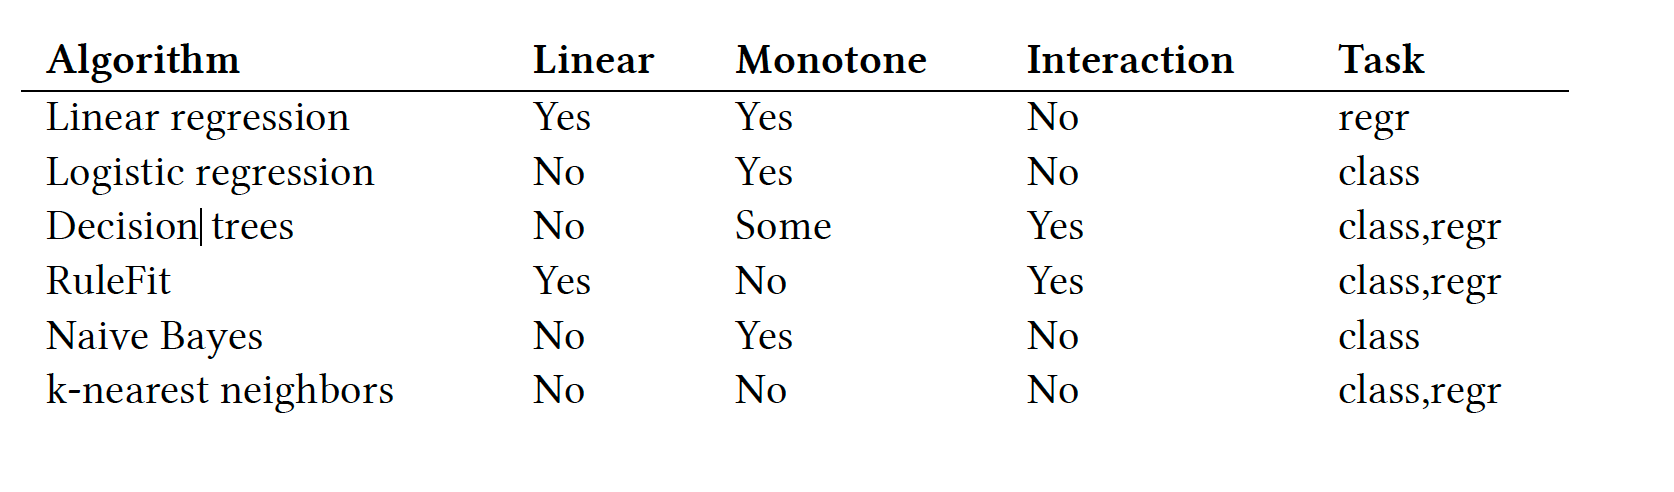
\includegraphics[width=0.7\textwidth]{img/int_models.png}
    \centering
\end{figure}
Some models allow to impose monotonicity and the possibility to include feature interactions.

\subsection{Linear Regression}
The dependent variable (target, prediction) is a weighted sum of the independent variables (predictors).
Linear models can be used to model the dependence of a regression target y on some features x. The learned relationships are linear and can be written for a single instance as follows:
\begin{equation}
    y=\beta_0+\beta_1x_1+\ldots+\beta_px_p+\epsilon
\end{equation}
The predicted outcome of an instance is a weighted sum of its $p$ features.
The betas ($\beta_j$) represent the learned feature weights or coefficients. 
The first weight in the sum ($\beta_0$) is called the intercept and is not multiplied with a feature.
The epsilon ($\epsilon$) is the error we still make, i.e. the difference between the prediction and the actual outcome. 
These errors are assumed to follow a Gaussian distribution, which means that we make errors in both negative and positive directions and make many small errors and few large errors.\\

Various methods can be used to estimate the optimal weight. The ordinary least squares method is usually used to find the weights that minimize the squared differences between the actual and the estimated outcomes:
\begin{equation}
    \hat{\boldsymbol{\beta}}=\arg\!\min_{\beta_0,\ldots,\beta_p}\sum_{i=1}^n\left(y^{(i)}-\left(\beta_0+\sum_{j=1}^p\beta_jx^{(i)}_{j}\right)\right)^{2}
\end{equation}

Estimated weights come with confidence intervals. A confidence interval is a range for the weight estimate that covers the “true” weight with a certain confidence. For example, a 95\% confidence interval for a weight of 
2 could range from 1 to 3. The interpretation of this interval would be: If we repeated the estimation 100 times with newly sampled data, the confidence interval would include the true weight in 95 out of 100 cases, given 
that the linear regression model is the correct model for the data.

Whether the model is the “correct” model depends on whether the relationships in the data meet certain assumptions:
\begin{itemize}
    \item \textbf{Linearity}: The linear regression model forces the
    prediction to be a linear combination of features, which is both its
    greatest strength and its greatest limitation. Linearity leads to
    interpretable models. Linear effects are easy to quantify and describe. They
    are additive, so it is easy to separate the effects. If you suspect feature
    interactions or a nonlinear association of a feature with the target value,
    you can add interaction terms or use regression splines.
    \item \textbf{Normality}: It is assumed that the target outcome given the features follows a normal distribution. If this assumption is violated, the estimated confidence intervals of the feature weights are invalid.
    \item \textbf{Homoscedasticity} (constant variance): The variance of the error terms is assumed to be constant over the entire feature space.
    \item \textbf{Independence}: It is assumed that each instance is independent of any other instance. If you perform repeated measurements, such as multiple blood tests per patient, the data points are not independent.
    \item \textbf{Fixed features}: The input features are considered “fixed”. Fixed means that they are treated as “given constants” and not as statistical variables. This implies that they are free of measurement errors.
    \item \textbf{Absence of multicollinearity}: You do not want strongly correlated features, because this messes up the estimation of the weights. In a situation where two features are strongly correlated, it becomes problematic to estimate the weights because the feature effects are additive and it becomes indeterminable to which of the correlated features to attribute the effects.
\end{itemize}

\subsubsection{Interpretation}
The interpretation of a weight in the linear regression model depends on the type of the corresponding feature.
\begin{itemize}
    \item \textbf{Numerical feature}: Increasing the numerical feature by one unit changes the estimated outcome by its weight.
    \item \textbf{Binary feature}: A feature that takes one of two possible values for each instance. Changing the feature from the reference category to the other category changes the estimated outcome by the feature's weight.
    \item \textbf{Intercept $\beta_0$}Changing the feature from the reference category to the other category changes the estimated outcome by the feature's weight.
    The interpretation of the intercept is usually not relevant because instances with all features values at zero often make no sense. The interpretation is only meaningful when the features have been standardised (mean of zero, standard deviation of one). Then the intercept reflects the predicted outcome of an instance where all features are at their mean value.
\end{itemize}

\subsubsection{Explained Variance}
Another important measurement for interpreting linear models is the R-squared measurement.
R-squared tells you how much of the total variance of your target outcome is explained by the model. The higher R-squared, the better your model explains the data. 
The formula for calculating R-squared is:
\begin{equation*}
    R^2=1-SSE/SST
\end{equation*}
SSE is the squared sum of the error terms:
\begin{equation*}
    SSE=\sum_{i=1}^n(y^{(i)}-\hat{y}^{(i)})^2
\end{equation*}
SST is the squared sum of the data variance:
\begin{equation*}
    SST=\sum_{i=1}^n(y^{(i)}-\bar{y})^2
\end{equation*}
The SSE tells you how much variance remains after fitting the linear model, which is measured by the squared differences between the predicted and actual target values.
SST is the total variance of the target outcome. R-squared tells you how much of your variance can be explained by the linear model. R-squared usually ranges between 0 
for models where the model does not explain the data at all and 1 for models that explain all of the variance in your data.\\

It is also possible for R-squared to take on a negative value without violating any mathematical rules.
This happens when SSE is greater than SST which means that a model does not capture the trend of the data and fits to the data worse than using the mean of the target as the prediction.\\

There is a catch, because R-squared increases with the number of features in the model, even if they do not contain any information about the target value at all. 
Therefore, it is better to use the adjusted R-squared, which accounts for the number of features used in the model. 
Its calculation is:
\begin{equation*}
    \bar{R}^2=1-(1-R^2)\frac{n-1}{n-p-1}
\end{equation*}
where p is the number of features and n the number of instances.

It is not meaningful to interpret a model with very low (adjusted) R-squared, because such a model basically does not explain much of the variance. Any interpretation of the weights would not be meaningful.

\subsubsection{Feature Importance}
The importance of a feature in a linear regression model can be measured by the absolute value of its t-statistic. 
The t-statistic is the estimated weight scaled with its standard error.
\begin{equation*}
    t_{\hat{\beta}_j}=\frac{\hat{\beta}_j}{SE(\hat{\beta}_j)}
\end{equation*}
Let us examine what this formula tells us: The importance of a feature increases with increasing weight. This makes sense.
The more variance the estimated weight has (= the less certain we are about the correct value), the less important the feature is. 
This also makes sense.
\subsubsection{Visual Interpretation}
Various visualizations make the linear regression model easy and quick to grasp for humans.\\

\textbf{Weight Plot}
The information of the weight table (weight and variance estimates) can be visualized in a weight plot. The following plot shows the results from the previous linear regression model.
\begin{figure}[H]
    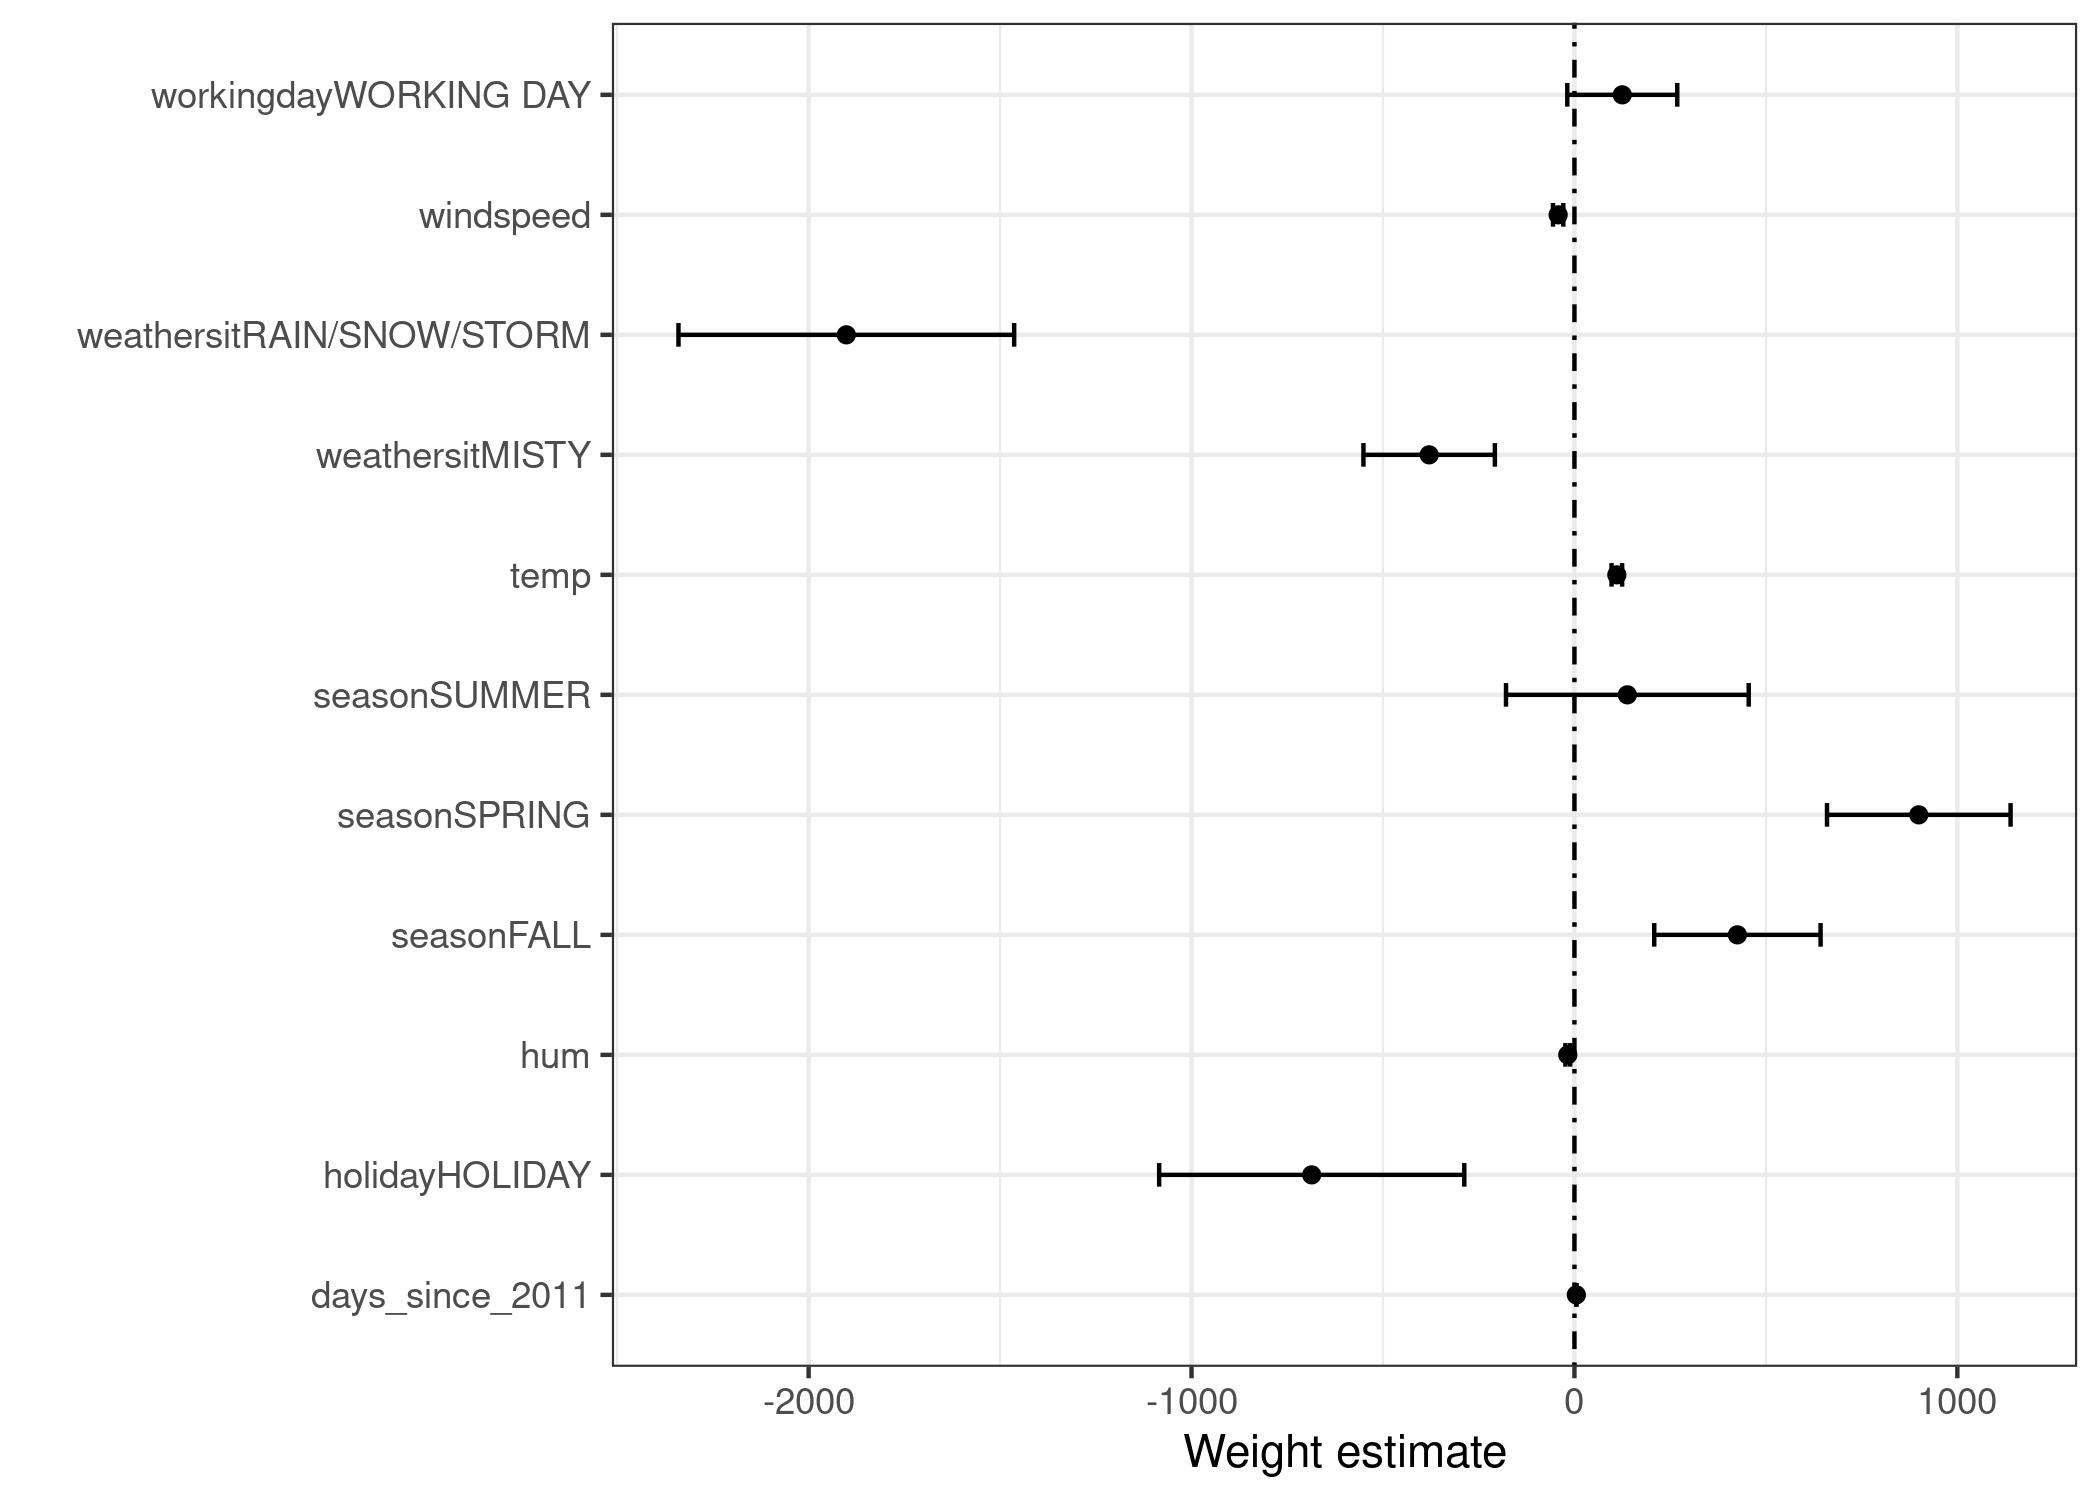
\includegraphics[width=0.5\textwidth]{img/linear-weights-plot-1.jpeg}
    \centering
\end{figure}
